\chapterimage{condprop.jpg}
\chapterspaceabove{6.75cm} 
\chapterspacebelow{8.25cm} 
\chapter{Conditional Probability and Independence of Events}

In this chapter, we will delve further into the realm of probability by introducing conditions that affect the occurrence of events. Conditional probability is not just a fundamental concept within the theory of probability; it is also crucial for understanding how the probability of events can be affected by the knowledge of the occurrence of other events. This concept is particularly important in fields such as statistics, finance, medicine, and many areas of science and engineering, where the likelihood of outcomes needs to be evaluated within a framework of known information.

The chapter will begin with a rigorous definition of conditional probability, followed by the derivation of the formula used to calculate it. We will explore examples that illustrate how conditional probability applies in various real-world scenarios, helping to clarify this seemingly abstract concept.

Additionally, we will discuss the concept of independence of events. Independence is a key notion that simplifies the computation of probabilities in situations where multiple events occur simultaneously. Understanding when events are independent, and when they are not, is crucial for correctly applying probabilistic models to real-life problems.

We will cover the following key topics in this chapter:
\begin{itemize}
    \item The definition and intuition behind conditional probability.
    \item The formula for conditional probability and how it is derived from the fundamental principles of probability.
    \item The Multiplication Rule for calculating the probability of the intersection of two events, based on conditional probability.
    \item The concept of independence, how it can be recognized, and its implications for the calculation of probabilities.
    \item Bayes's Theorem, a pivotal result in probability that relies on the concept of conditional probability to reverse conditional relationships.
    \item Practical applications and examples that demonstrate the use and impact of conditional probability and independence in various fields.
\end{itemize}
\
Through the exploration of these topics, the chapter aims to provide a comprehensive understanding of how probabilities are adjusted based on conditions and dependencies between events, equipping you with the analytical tools necessary for tackling complex probabilistic scenarios. We will conclude the chapter with exercises that reinforce these concepts and challenge you to apply what you have learned in theoretical and practical contexts.

\section{Conditional Probability}
We first introduce probability with conditions. Like its verbatim meaning, conditional probabilities are obtained by adding constraints to existing probability. Essentially, when we 
are trying to find conditional probability, we are looking for a new probability in from a compressed sample space.
\begin{definition}[Conditional Probability]
    Given two events, \(A\) and \(B\), in a probability space, with \(P(B) > 0\), the conditional probability of \(A\) given \(B\) is defined by the formula:
    \[
    P(A \mid B) = \frac{P(A \cap B)}{P(B)},
    \]
    where \(P(A \cap B)\) is the probability of the intersection of \(A\) and \(B\), and \(P(B)\) is the probability of \(B\).
    \end{definition}
\begin{remark}
    This definition assumes that \(P(B) > 0\), because conditional probability is undefined when \(P(B) = 0\). The definition essentially describes how the likelihood of \(A\) is adjusted by the occurrence of \(B\), providing a way to update beliefs about the likelihood of an event based on new information about another event.
\end{remark}
\begin{proof}
    We need to demonstrate that the definition of \( P(E \mid F) \) as \( \frac{P(EF)}{P(F)} \) is logically consistent and adheres to the axioms of probability.
    
    Let's consider the sample space \(\Omega\), where \( F \subseteq \Omega \) and \( P(F) > 0 \). By definition, \( EF \) is the event where both \( E \) and \( F \) occur. We want to compute \( P(E \mid F) \), the probability of \( E \) occurring given that \( F \) has occurred.
    
    \textbf{Step 1: Relative Frequency Interpretation}
    In the relative frequency interpretation of probability, if we were to repeat an experiment a large number of times, \( P(F) \) would be the proportion of times that event \( F \) occurs, and \( P(EF) \) would be the proportion of times both events \( E \) and \( F \) occur together.
    
    \textbf{Step 2: Conditional Probability Calculation}
    Given that \( F \) has occurred, the new sample space is restricted to \( F \). Hence, we need to adjust all probabilities to this new sample space. The probability of any event \( E \) in this new sample space (i.e., under the condition \( F \)) is the proportion of \( F \) that also belongs to \( E \), which is exactly \( EF \). Thus,
    \[
    P(E \mid F) = \frac{\text{Number of outcomes in } EF}{\text{Number of outcomes in } F} = \frac{P(EF)}{P(F)}
    \]
    
    Therefore, the definition \( P(E \mid F) = \frac{P(EF)}{P(F)} \) is a valid and logical extension of the probability measure to the conditioned space where \( F \) has occurred.
    \end{proof}
    
We illustrate this with an example from dice again.

\begin{example}[Rolling a Die Twice]
Consider the experiment of rolling a fair six-sided die twice. We are interested in the conditional probability of the sum of the numbers on the two dice being greater than 8, given that the first die shows a 4.

\subsubsection*{Sample Space Representation}
The total sample space when rolling a die twice can be represented by a lattice diagram, where each point \((x,y)\) corresponds to the outcome where the first roll results in \(x\) and the second roll results in \(y\).

% Drawing the lattice diagram for the sample space
\begin{center}
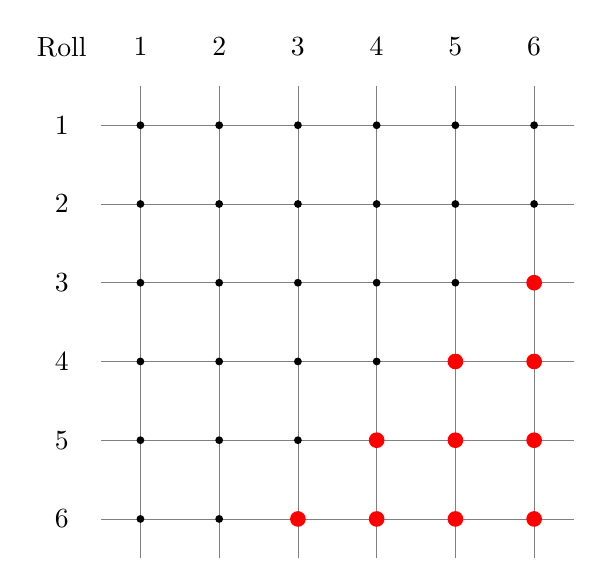
\begin{tikzpicture}[scale=1]
    % Draw grid
    \draw[step=1cm,gray,very thin] (0.5,0.5) grid (6.5,6.5);
    
    % Label rows and columns
    \foreach \x in {1,...,6} {
        \foreach \y in {1,...,6} {
            \node at (\x, 7-\y) [circle, fill, inner sep=1pt]{};
        }
        \node at (\x, 7) {\x}; % Top labels
    }
    \foreach \y in {1,...,6} {
        \node at (0, 7-\y) {\y}; % Side labels
    }
    
    % Color cells where the sum is greater than 8
    \foreach \x in {1,...,6} {
        \foreach \y in {1,...,6} {
            \pgfmathtruncatemacro{\result}{\x + \y}
            \ifnum \result>8
                \node at (\x, 7-\y) [circle, fill=red, inner sep=2pt]{};
            \fi
        }
    }
    \node at (0,7) {Roll};
\end{tikzpicture}
\end{center}

\subsubsection*{Event \(B\): First Roll is a 4}
Given the event \(B\) that the first die roll results in a 4, we focus on the fourth column of the lattice diagram, and the outcomes that contribute to \(A \cap B\) are highlighted.

% Drawing the reduced sample space for B
\begin{center}
\begin{tikzpicture}[scale=1]
    % Draw specific column for roll=4
    \draw[step=1cm,gray,very thin] (3.5,0.5) grid (4.5,6.5);
    
    % Label column and rows
    \foreach \y in {1,...,6} {
        \node at (4, 7-\y) [circle, fill, inner sep=1pt]{};
        \node at (0, 7-\y) {\y}; % Side labels
    }
    
    % Color cells where the sum is greater than 8 with the first roll = 4
    \foreach \y in {1,...,6} {
        \pgfmathtruncatemacro{\result}{4 + \y}
        \ifnum \result>8
            \node at (4, 7-\y) [circle, fill=red, inner sep=2pt]{};
        \fi
    }
    \node at (0,7) {Roll};
    \node at (4,7) {4}; % Label for the first roll
\end{tikzpicture}
\end{center}

\subsubsection*{Conditional Probability \(P(A \mid B)\)}
With \(B\) set as the first roll being 4, \(A \cap B\) involves outcomes (4,5) and (4,6), making \(P(A \cap B) = \frac{2}{36} = \frac{1}{18}\), and \(P(B) = \frac{6}{36} = \frac{1}{6}\).

Hence, the conditional probability is calculated as:
\[
P(A \mid B) = \frac{P(A \cap B)}{P(B)} = \frac{\frac{1}{18}}{\frac{1}{6}} = \frac{1}{3}.
\]
\begin{remark}
    This result is equivalent to $\frac{2}{6}=\frac{1}{3}$ in the subspace, we just use the measurement from the original sample space for clarity.
    So both explainations are acceptable, while the other one is more understandable when you cannot show the subspace.
\end{remark}
\end{example}

With this example, I believe that you must know how conditional probability is all about. However, this is only a very special case. 
You may have noticed that for rolling a fair dice, we have equal possibility to get 1-6 in each roll. In the real life, most events have different probabilities. Let's see another example of unfaired dice.
But to solve this problem, we need to use an important conclusion of conditional probability.
\begin{corollary}\label{intersectascond}
    By multiplying $P(F)$ to \( P(E \mid F) = \frac{P(EF)}{P(F)} \), we find that 
    \begin{equation}\label{intasprob}
        P(EF) = P(E \mid F)P(F)
    \end{equation}
\end{corollary}
\begin{example}\label{unfair_dice}
    An unfair four-sided die (numbered 1 to 4) is rolled twice. The biases for the die are:
    \begin{itemize}
        \item \( P(1) = 0.1 \)
        \item \( P(2) = 0.2 \)
        \item \( P(3) = 0.3 \)
        \item \( P(4) = 0.4 \)
    \end{itemize}
    We are tasked with calculating:
    \begin{enumerate}
        \item The conditional probability that the sum of the two rolls is 4, given that the first roll is a 2.
        \item The conditional probability that the first roll is a 2, given that the sum of the two rolls is 4.
    \end{enumerate}
\end{example}
\begin{solution}
    Define the events:
    \begin{itemize}
        \item \( A \): The sum of the two rolls is 4.
        \item \( B \): The first roll is a 2.
    \end{itemize}
    We can draw a tree diagram to show all possible results with possibility of each branch.
    \begin{center}
        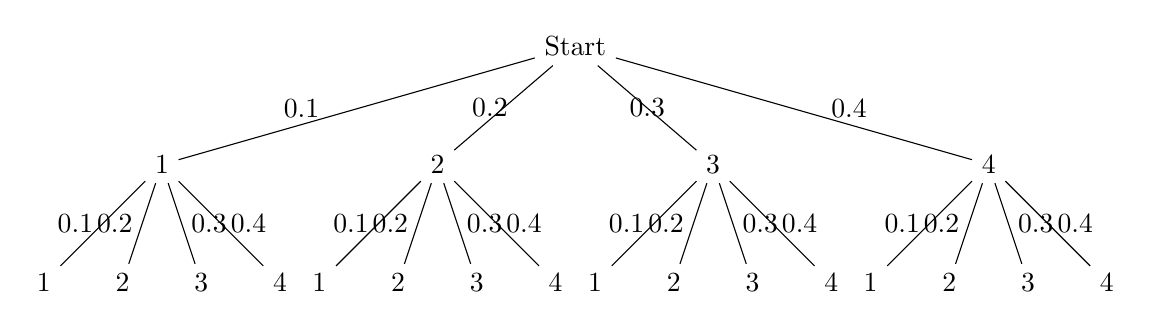
\begin{tikzpicture}[scale=1, every node/.style={align=center}, level distance=1.5cm,
          level 1/.style={sibling distance=3.5cm},
          level 2/.style={sibling distance=1cm}]
            % Level 1
            \node {Start}
                child {node {1}
                    child {node {1} edge from parent node[left] {0.1}}
                    child {node {2} edge from parent node[left] {0.2}}
                    child {node {3} edge from parent node[right] {0.3}}
                    child {node {4} edge from parent node[right] {0.4}}
                    edge from parent node[left, xshift=-10] {0.1}
                }
                child {node {2}
                    child {node {1} edge from parent node[left] {0.1}}
                    child {node {2} edge from parent node[left] {0.2}}
                    child {node {3} edge from parent node[right] {0.3}}
                    child {node {4} edge from parent node[right] {0.4}}
                    edge from parent node[left, xshift=5] {0.2}
                }
                child {node {3}
                    child {node {1} edge from parent node[left] {0.1}}
                    child {node {2} edge from parent node[left] {0.2}}
                    child {node {3} edge from parent node[right] {0.3}}
                    child {node {4} edge from parent node[right] {0.4}}
                    edge from parent node[left, xshift=10] {0.3}
                }
                child {node {4}
                    child {node {1} edge from parent node[left] {0.1}}
                    child {node {2} edge from parent node[left] {0.2}}
                    child {node {3} edge from parent node[right] {0.3}}
                    child {node {4} edge from parent node[right] {0.4}}
                    edge from parent node[right, xshift=10] {0.4}
                };
        \end{tikzpicture}
        \end{center}
    \subsubsection*{1. \( P(A \mid B) \)}
    The event \( B \) fixes the first roll at 2. For \( A \) to occur with \( B \), the second roll must be 2 (i.e., \( 2 + 2 = 4 \)).
    \[ P(A \mid B) = P(\text{Second roll is 2}) = P(2) = 0.2 \]
    This could also easily be examined from the graph the 2-2 is the only branch among the four possible cases under 2 in the first roll, so we have $P(A \mid B) = \frac{0.2\times 0.2}{0.2}=0.2$.
    \begin{remark}
        We get $P(A \mid B) = \frac{0.2\times 0.2}{0.2}=0.2$ by using the corollary to the numerator, which is the probability of getting a two twice. 
        By the corollary, it can be expressed as the product of the probability we get 2 in the second trial given that 2 is ontained in the first attempt, and $P(2)$.
        It is obvious that the condition does not work here, because we always have the same chance of getting a 2. Thus we have $0.2^2$ as the numerator of $P(A \mid B)$.
    \end{remark}
    \subsubsection*{2. \( P(B \mid A) \)}
    The event \( A \) (sum is 4) can occur through the following combinations:
    \begin{itemize}
        \item \( (1, 3) \) and \( (3, 1) \)
        \item \( (2, 2) \)
    \end{itemize}
    
    Calculate \( P(A) \):
    \[ P(A) = P(1, 3) + P(3, 1) + P(2, 2) = 0.1 \cdot 0.3 + 0.3 \cdot 0.1 + 0.2 \cdot 0.2 = 0.03 + 0.03 + 0.04 = 0.1 \]
    \begin{remark}
        Note that we use Eq \ref{intasprob} here, since for some event $E,F$, $P(E\cap F) = P(E \mid F)P(F)$.
        We get the probability of each branch by using the RHS of the equation using the probability on the edge of the tree 
        diagram. E.g., we have 3 for the second roll and 1 in the first roll, then we have $0.3\times 0.1 = 0.03$ chance for the coresponding result.
        Note that the weight on the tree graph in every layer are treated as conditional probability, and 0.3 is the probability of a three given that the first roll gives 1
    \end{remark}
    Now, \( P(B \mid A) \):
    \[ P(B \mid A) = \frac{P(B \cap A)}{P(A)} = \frac{P(2, 2)}{P(A)} = \frac{0.04}{0.1} = 0.4 \]
    
 From this example we see that despite that we have different probability for each branch of events, what we are doing to find conditional probability is still the same:
 subsetting the sample space and locate our target cases in that subspace.
\end{solution}

We wrap up the use of lattice diagram and tree diagram here.
    \subsubsection*{Lattice Diagram}
    Lattice diagrams are particularly useful for representing all possible outcomes in a sequence of events where outcomes are straightforward and often \textbf{uniformly distributed}, such as 
    flipping coins or rolling dice. They are excellent for visualizing permutations, combinations, and the structure of outcomes in multi-stage experiments. A lattice diagram efficiently showcases how different
    paths can lead to various results, making it ideal for illustrating scenarios with equal probabilities or for modeling situations like financial derivatives pricing, where the path dependencies of 
    options or other financial instruments are important.
    \subsubsection*{Tree Diagram}
    Tree diagrams, on the other hand, excel in situations where outcomes have different probabilities(i.e., \textbf{not uniformly distributed} ) or the process is inherently hierarchical. They are invaluable for breaking down complex probability problems into 
    manageable parts, especially in Bayesian statistics where updates to probability estimates are made as new information becomes available. Tree diagrams allow for the visualization of conditional probabilities 
    and sequential decision processes, making them perfect for scenarios where events are dependent on previous outcomes, such as sequential games, Bayesian inference, or decision analysis.

    But of course, we will not always use diagram for problem-solving, since you can imagine how complex the diagram could be when the scale of the problem increases. Fundamentally,
    we still need to obtain the result by analyzing the chain of events and their relations with the given conditions in different contexts.

    Here are some more interesting examples.

    \begin{example}
        Celine is undecided whether to take a French course or a chemistry course. She estimates that her probability of receiving an A grade would be \(\frac{1}{2}\) in a French course and \(\frac{2}{3}\) in a chemistry course. If Celine decides to base her decision on the flip of a fair coin, what is the probability that she gets an A in chemistry?
        \end{example}
        
        \begin{solution}
        Let \( C \) be the event that Celine takes the chemistry course and \( A \) be the event that she receives an A in whatever course she takes. The decision to take chemistry is based on the flip of a fair coin, thus \( P(C) = \frac{1}{2} \).
        
        Given \( C \) (the event of taking chemistry), the probability of \( A \) (receiving an A) in chemistry is \( P(A \mid C) = \frac{2}{3} \). Therefore, the probability that Celine takes chemistry and gets an A can be calculated using the rule of multiplication for probabilities:
        
        \[
        P(CA) = P(C)P(A \mid C) = \left(\frac{1}{2}\right)\left(\frac{2}{3}\right) = \frac{1}{3}.
        \]
        
        Thus, the probability that Celine gets an A in chemistry, given that her decision is based on a coin flip, is \(\frac{1}{3}\).
        \end{solution}
        \begin{remark}
        Some people may wonder why we are calculating probability of intersection instead of conditional probability here. Because semantically, the probability of getting A in chemistry
        \textbf{given that} we get head/tail of the coin seems equivalent to the probability of getting A in chemistry, \textbf{and} we get head/tail of the coin. The answer if completely NO.
        Because when we gauge the conditional probability, condition(s) matters. Will the result of flipping the coin affact the chance of getting A in chemistry? Of course no, so we are not finding
        a conditional probability. We will discuss this further in independence of events. This is a vivid example that demonstrates the difference of sumbolic language and natural language. The former
        outperforms in terms of accuracy but less understandable for human, while natural language is more understandable but in many cases, bring a lot of bias.
        \end{remark}

        \begin{example}
            Suppose that an urn contains 8 red balls and 4 white balls. We draw 2 balls from the urn without replacement.
            
            \textbf{(a)} If we assume that at each draw, each ball in the urn is equally likely to be chosen, what is the probability that both balls drawn are red?
            
            \textbf{(b)} Now suppose that the balls have different weights, with each red ball having weight \(r\) and each white ball having weight \(w\). Suppose that the probability that a given ball in the urn is the next one selected is its weight divided by the sum of the weights of all balls currently in the urn. Now what is the probability that both balls are red?
            \end{example}
            
            \begin{solution}
            \textbf{(a)} Let \( R_1 \) and \( R_2 \) denote, respectively, the events that the first and second balls drawn are red. Given that the first ball selected is red, there are 7 remaining red balls and 4 white balls, so \( P(R_2|R_1) = \frac{7}{11} \). As \( P(R_1) \) is clearly \(\frac{8}{12}\), the desired probability is calculated as:
            \[
            P(R_1 R_2) = P(R_1)P(R_2|R_1) = \left(\frac{2}{3}\right)\left(\frac{7}{11}\right) = \frac{14}{33}.
            \]
            
            \textbf{(b)} For this part, we again let \( R_i \) be the event that the \(i\)-th ball chosen is red and use:
            \[
            P(R_1 R_2) = P(R_1)P(R_2|R_1)
            \]
            Now, number the red balls, and let \( B_i, i = 1, \ldots, 8 \) be the event that the first ball drawn is red ball number \( i \). Then:
            \[
            P(R_1) = P\left(\bigcup_{i=1}^8 B_i\right) = \sum_{i=1}^8 P(B_i) = \frac{8r}{8r + 4w}
            \]
            Moreover, given that the first ball is red, the urn then contains 7 red and 4 white balls. Thus, by a similar argument:
            \[
            P(R_2|R_1) = \frac{7r}{7r + 4w}
            \]
            Hence, the probability that both balls are red is:
            \[
            P(R_1 R_2) = \frac{8r}{8r + 4w} \times \frac{7r}{7r + 4w} = \frac{8r \times 7r}{(8r + 4w)(7r + 4w)}
            \]
            \end{solution}
    
        Now let's move further onto the generalization of corollary \ref{intersectascond}, known as The multiplication rule of probability.
        \begin{theorem}[Multiplication Rule]
            If \(E_1, E_2, \ldots, E_n\) are events, then the probability of all these events occurring in sequence is given by:
            \[
            P(E_1 E_2 \cdots E_n) = P(E_1) P(E_2 \mid E_1) P(E_3 \mid E_1 E_2) \cdots P(E_n \mid E_1 E_2 \cdots E_{n-1})
            \]
            \end{theorem}
            
            \begin{proof}
            We prove the theorem by induction on the number of events \(n\).
            
            \textbf{Base case} (\(n = 2\)): For two events \(E_1\) and \(E_2\), the multiplication rule reduces to:
            \[
            P(E_1 E_2) = P(E_1) P(E_2 \mid E_1),
            \]
            which is the definition of the conditional probability of \(E_2\) given \(E_1\).
            
            \textbf{Inductive step}: Assume that the theorem holds for \(n-1\) events. That is, we assume:
            \[
            P(E_1 E_2 \cdots E_{n-1}) = P(E_1) P(E_2 \mid E_1) \cdots P(E_{n-1} \mid E_1 \cdots E_{n-2}).
            \]
            We need to prove that the rule holds for \(n\) events. By the definition of conditional probability, we have:
            \[
            P(E_1 E_2 \cdots E_n) = P(E_1 E_2 \cdots E_{n-1}) P(E_n \mid E_1 E_2 \cdots E_{n-1}).
            \]
            Applying the induction hypothesis, we substitute for \(P(E_1 E_2 \cdots E_{n-1})\):
            \[
            P(E_1 E_2 \cdots E_n) = \left(P(E_1) P(E_2 \mid E_1) \cdots P(E_{n-1} \mid E_1 \cdots E_{n-2})\right) P(E_n \mid E_1 \cdots E_{n-1}),
            \]
            which confirms the theorem for \(n\) events.
            
            Thus, by the principle of mathematical induction, the multiplication rule holds for any number of events.
        \end{proof}
        \begin{remark}
            Actually, we have a more decent way to prove it, which works like chain rule in differentiation.To prove the multiplication rule, just apply the definition of conditional probability
            to its right-hand side, giving
            \[P(E_1)\frac{P(E_1E_2)}{P(E_1)}\frac{P(E_1E_2E_3)}{P(E_1E_2)}\cdots\frac{P(E_1E_2\cdots E_n)}{P(E_1E_2\cdots E_{n-1})}=P(E_1E_2\cdots E_n)\]
        \end{remark}
\section{Bayes's Theorem}

\section{Further Conditional Probability}

\section{Independence of Events}